%---------------------------------------------------------------------
\section{Resultados das simula��es}

Simula��o utilizando \HI{\texttt{Matlab/Simulink}}.

\subsection{Simula��o \#1}

\bigskip%
Par�metros e condi��es iniciais  :
%
\begin{align*}
  a_p &= -2\,,  &  y_p(0) &= 0\,, & \theta(0) &= 0\,, \\
  a_m &= 1\,,   &  y_m(0) &= 0\,, & \gamma &= 2,\ 100\,, \\
  r &= 1\,, & a_f &= 1\,.
\end{align*}

\bigskip%
\begin{figure}[H]
  \centering
  \includegraphics[width=12cm]{figs/e0_vs_deltatheta/ap-2am1yp00af1.eps} \\[2mm]
  \caption{Diagrama $e_0 \times \tilde{\theta}$.}
\end{figure}

\newpage%
%---------------------------------------------------------------------
\begin{figure}[H]
  \centering
  \includegraphics[width=12cm]{figs/e0/ap-2am1yp00af1.eps}
\end{figure}

\begin{figure}[H]
  \centering
  \includegraphics[width=12cm]{figs/theta/ap-2am1yp00af1.eps} 
\end{figure}

\begin{figure}[H]
  \centering
  \includegraphics[width=12cm]{figs/u/ap-2am1yp00af1.eps} 
\end{figure}

\begin{figure}[H]
  \centering
  \includegraphics[width=12cm]{figs/yp/ap-2am1yp00af1.eps} 
\end{figure}

\newpage%
%---------------------------------------------------------------------
\subsection{Simula��o \#2}

\bigskip%
Par�metros e condi��es iniciais  :
%
\begin{align*}
  a_p &= -2\,,  &  y_p(0) &= \HI{2}\,, & \theta(0) &= 0\,, \\
  a_m &= 1\,,   &  y_m(0) &= 0\,, & \gamma &= 2,\ 100\,, \\
  r &= 1\,, & a_f &= 1\,.
\end{align*}

\bigskip%
\begin{figure}[H]
  \centering
  \includegraphics[width=12cm]{figs/e0_vs_deltatheta/ap-2am1yp02af1.eps} \\[2mm]
  \caption{Diagrama $e_0 \times \tilde{\theta}$.}
\end{figure}

%---------------------------------------------------------------------
\begin{figure}[H]
  \centering
  \includegraphics[width=12cm]{figs/e0/ap-2am1yp02af1.eps} 
\end{figure}

\begin{figure}[H]
  \centering
  \includegraphics[width=12cm]{figs/theta/ap-2am1yp02af1.eps} 
\end{figure}

\begin{figure}[H]
  \centering
  \includegraphics[width=12cm]{figs/u/ap-2am1yp02af1.eps} 
\end{figure}

\begin{figure}[H]
  \centering
  \includegraphics[width=12cm]{figs/yp/ap-2am1yp02af1.eps} 
\end{figure}

\newpage%
%---------------------------------------------------------------------
\subsection{Simula��o \#3}

\bigskip%
Par�metros e condi��es iniciais  :
%
\begin{align*}
  a_p &= -2\,,  &  y_p(0) &= \HI{10}\,, & \theta(0) &= 0\,, \\
  a_m &= 1\,,   &  y_m(0) &= 0\,, & \gamma &= 2,\ 100\,, \\
  r &= 1\,, & a_f &= 1\,.
\end{align*}

\bigskip%
\begin{figure}[H]
  \centering
  \includegraphics[width=12cm]{figs/e0_vs_deltatheta/ap-2am1yp010af1.eps}
  \\[2mm] \caption{Diagrama $e_0 \times \tilde{\theta}$.}
\end{figure}

\newpage%
%---------------------------------------------------------------------
\begin{figure}[H]
  \centering
  \includegraphics[width=12cm]{figs/e0/ap-2am1yp010af1.eps} 
\end{figure}

\begin{figure}[H]
  \centering
  \includegraphics[width=12cm]{figs/theta/ap-2am1yp010af1.eps} 
\end{figure}

\begin{figure}[H]
  \centering
  \includegraphics[width=12cm]{figs/u/ap-2am1yp010af1.eps} 
\end{figure}

\begin{figure}[H]
  \centering
  \includegraphics[width=12cm]{figs/yp/ap-2am1yp010af1.eps} 
\end{figure}
\newpage%
%---------------------------------------------------------------------

\subsection{Simula��o \#4}

\bigskip%
Par�metros e condi��es iniciais  :
%
\begin{align*}
  a_p &= \HI{-10}\,,  &  y_p(0) &= 0\,, & \theta(0) &= 0\,, \\
  a_m &= 1\,,   &  y_m(0) &= 0\,, & \gamma &= 2,\ 100\,, \\
  r &= 1\,, & a_f &= 1\,.
\end{align*}

\bigskip%
\begin{figure}[H]
  \centering
  \includegraphics[width=12cm]{figs/e0_vs_deltatheta/ap-10am1yp00af1.eps}
  \\[2mm] \caption{Diagrama $e_0 \times \tilde{\theta}$.}
\end{figure}

\newpage%
%---------------------------------------------------------------------
\begin{figure}[H]
  \centering
  \includegraphics[width=12cm]{figs/e0/ap-10am1yp00af1.eps} 
\end{figure}

\begin{figure}[H]
  \centering
  \includegraphics[width=12cm]{figs/theta/ap-10am1yp00af1.eps} 
\end{figure}

\begin{figure}[H]
  \centering
  \includegraphics[width=12cm]{figs/u/ap-10am1yp00af1.eps} 
\end{figure}

\begin{figure}[H]
  \centering
  \includegraphics[width=12cm]{figs/yp/ap-10am1yp00af1.eps} 
\end{figure}
\newpage%

%---------------------------------------------------------------------

\subsection{Simula��o \#5}

\bigskip%
Par�metros e condi��es iniciais  :
%
\begin{align*}
  a_p &= -2\,,  &  y_p(0) &= 0\,, & \theta(0) &= 0\,, \\
  a_m &= \HI{10}\,,   &  y_m(0) &= 0\,, & \gamma &= 2,\ 100\,, \\
  r &= 1\,, & a_f &= \HI{10}\,.
\end{align*}

\bigskip%
\begin{figure}[H]
  \centering
  \includegraphics[width=12cm]{figs/e0_vs_deltatheta/ap-2am10yp00af10.eps}
  \\[2mm] \caption{Diagrama $e_0 \times \tilde{\theta}$.}
\end{figure}

\newpage%
%---------------------------------------------------------------------
\begin{figure}[H]
  \centering
  \includegraphics[width=12cm]{figs/e0/ap-2am10yp00af10.eps} 
\end{figure}

\begin{figure}[H]
  \centering
  \includegraphics[width=12cm]{figs/theta/ap-2am10yp00af10.eps} 
\end{figure}

\begin{figure}[H]
  \centering
  \includegraphics[width=12cm]{figs/u/ap-2am10yp00af10.eps} 
\end{figure}

\begin{figure}[H]
  \centering
  \includegraphics[width=12cm]{figs/yp/ap-2am10yp00af10.eps} 
\end{figure}
\newpage%

%---------------------------------------------------------------------

\subsection{Simula��o \#6}

\bigskip%
Par�metros e condi��es iniciais  :
%
\begin{align*}
  a_p &= -2\,,  &  y_p(0) &= 0\,, & \theta(0) &= 0\,, \\
  a_m &= 1\,,   &  y_m(0) &= 0\,, & \gamma &= 2,\ 100\,, \\
  r &= 1\,, & a_f &= \HI{0.5}\,.
\end{align*}

\bigskip%
\begin{figure}[H]
  \centering
  \includegraphics[width=12cm]{figs/e0_vs_deltatheta/ap-2am1yp00af05.eps}
  \\[2mm] \caption{Diagrama $e_0 \times \tilde{\theta}$.}
\end{figure}

\newpage%
%---------------------------------------------------------------------
\begin{figure}[H]
  \centering
  \includegraphics[width=12cm]{figs/e0/ap-2am1yp00af05.eps} 
\end{figure}

\begin{figure}[H]
  \centering
  \includegraphics[width=12cm]{figs/theta/ap-2am1yp00af05.eps} 
\end{figure}

\begin{figure}[H]
  \centering
  \includegraphics[width=12cm]{figs/u/ap-2am1yp00af05.eps} 
\end{figure}

\begin{figure}[H]
  \centering
  \includegraphics[width=12cm]{figs/yp/ap-2am1yp00af05.eps} 
\end{figure}
\newpage%

%---------------------------------------------------------------------

\subsection{Simula��o \#7}

\bigskip%
Par�metros e condi��es iniciais  :
%
\begin{align*}
  a_p &= -2\,,  &  y_p(0) &= 0\,, & \theta(0) &= 0\,, \\
  a_m &= 1\,,   &  y_m(0) &= 0\,, & \gamma &= 2,\ 100\,, \\
  r &= 1\,, & a_f &= \HI{10}\,.
\end{align*}

\bigskip%
\begin{figure}[H]
  \centering
  \includegraphics[width=12cm]{figs/e0_vs_deltatheta/ap-2am1yp00af10.eps}
  \\[2mm] \caption{Diagrama $e_0 \times \tilde{\theta}$.}
\end{figure}

\newpage%
%---------------------------------------------------------------------
\begin{figure}[H]
  \centering
  \includegraphics[width=12cm]{figs/e0/ap-2am1yp00af10.eps} 
\end{figure}

\begin{figure}[H]
  \centering
  \includegraphics[width=12cm]{figs/theta/ap-2am1yp00af10.eps} 
\end{figure}

\begin{figure}[H]
  \centering
  \includegraphics[width=12cm]{figs/u/ap-2am1yp00af10.eps} 
\end{figure}

\begin{figure}[H]
  \centering
  \includegraphics[width=12cm]{figs/yp/ap-2am1yp00af10.eps} 
\end{figure}
\newpage%

%---------------------------------------------------------------------

\subsection{Simula��o \#8}

\bigskip%
Par�metros e condi��es iniciais  :
%
\begin{align*}
  a_p &= -2\,,  &  y_p(0) &= 0\,, & \theta(0) &= 0\,, \\
  a_m &= 1\,,   &  y_m(0) &= 0\,, & \gamma &= 2,\ 100\,, \\
  r &= 1\,, & a_f &= \HI{5}\,.
\end{align*}

\bigskip%
\begin{figure}[H]
  \centering
  \includegraphics[width=12cm]{figs/e0_vs_deltatheta/ap-2am1yp00af5.eps}
  \\[2mm] \caption{Diagrama $e_0 \times \tilde{\theta}$.}
\end{figure}

\newpage%
%---------------------------------------------------------------------
\begin{figure}[H]
  \centering
  \includegraphics[width=12cm]{figs/e0/ap-2am1yp00af5.eps} 
\end{figure}

\begin{figure}[H]
  \centering
  \includegraphics[width=12cm]{figs/theta/ap-2am1yp00af5.eps} 
\end{figure}

\begin{figure}[H]
  \centering
  \includegraphics[width=12cm]{figs/u/ap-2am1yp00af5.eps} 
\end{figure}

\begin{figure}[H]
  \centering
  \includegraphics[width=12cm]{figs/yp/ap-2am1yp00af5.eps} 
\end{figure}
\newpage%

%---------------------------------------------------------------------

\subsection{Simula��o \#9}

\bigskip%
Par�metros e condi��es iniciais  :
%
\begin{align*}
  a_p &= \HI{-10}\,,  &  y_p(0) &= 0\,, & \theta(0) &= 0\,, \\
  a_m &= \HI{5}\,,   &  y_m(0) &= 0\,, & \gamma &= 2,\ 100\,, \\
  r &= 1\,, & a_f &= \HI{5}\,.
\end{align*}

\bigskip%
\begin{figure}[H]
  \centering
  \includegraphics[width=12cm]{figs/e0_vs_deltatheta/ap-10am5yp00af5.eps}
  \\[2mm] \caption{Diagrama $e_0 \times \tilde{\theta}$.}
\end{figure}

\newpage%
%---------------------------------------------------------------------
\begin{figure}[H]
  \centering
  \includegraphics[width=12cm]{figs/e0/ap-10am5yp00af5.eps} 
\end{figure}

\begin{figure}[H]
  \centering
  \includegraphics[width=12cm]{figs/theta/ap-10am5yp00af5.eps} 
\end{figure}

\begin{figure}[H]
  \centering
  \includegraphics[width=12cm]{figs/u/ap-10am5yp00af5.eps} 
\end{figure}

\begin{figure}[H]
  \centering
  \includegraphics[width=12cm]{figs/yp/ap-10am5yp00af5.eps} 
\end{figure}
\newpage%